%!TEX root = ../thesis.tex

\chapter{Similarity Measures} % Main chapter title

\label{chapter:Measures} % Change X to a consecutive number; for referencing this chapter elsewhere, use \ref{ChapterX}

\lhead{Chapter 4 \emph{Semantic Similarity Measures}} % Change X to a consecutive number; this is for the header on each page - perhaps a shortened title

This chapter aims to review several similarity measures. The first two sections describe semantic metrics when the last one shortly present a statistical way to measure concepts' relatedness. In order to illustrate those methods, we will used the figure \ref{fig:ontology} which is an handcrafted ontology.

\begin{figure}[!h]
\begin{center}
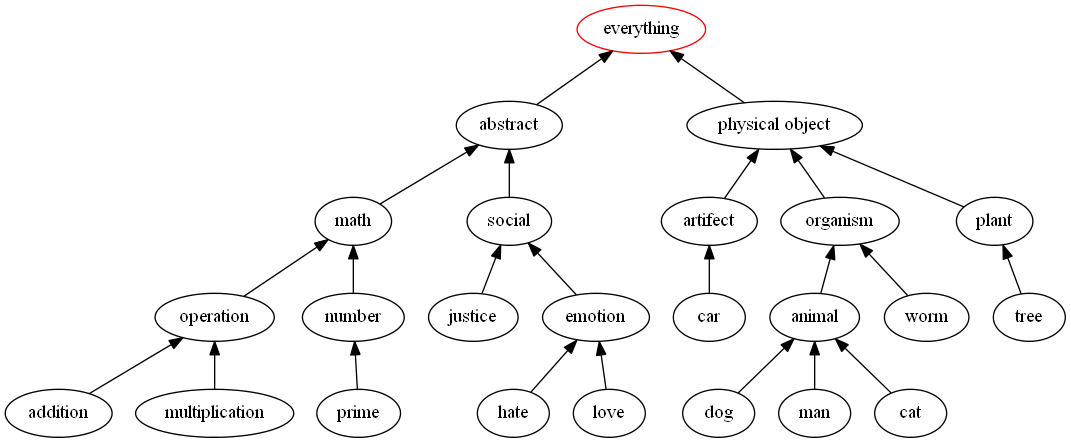
\includegraphics[width=0.90\textwidth]{./Primitives/ontology-handcraft-example.png}
\end{center}
\caption{Sample ontology}
\label{fig:ontology}
\end{figure}

%----------------------------------------------------------------------------------------
%	SECTION 1
%----------------------------------------------------------------------------------------

\section{Edge-based}

\subsection{Shortest Path} % (fold)
\label{ssub:shortest_path}
This measure is in fact a simple node-counting scheme (path). The similarity score is inversely proportional to the number of nodes along the shortest path between the concepts. The shortest possible path occurs when the two concepts are the same, in which case the length is 1. Thus, the maximum similarity value is 1.\\

One has to be very careful with the use of this metric because it initially doesn't take into account neither the kind of relations nor their direction. Therefore, two concepts which are hierarchically related may be as similar as two leafs. Based on figure \ref{fig:ontology} we can for instance see that :
\begin{equation}
\label{eq:shortpath}
sim_{SP}(addition, social) = sim_{SP}(addition, prime) = 1/4 = 0.25
\end{equation}
It means that, with regards to the Shortest Path metric, addition and social are as similar as addition and prime.
% subsection shortest_path (end)

\subsection{Wu-Palmer} % (fold)
\label{ssub:wu_palmer}
In \cite{wu1994verbs} Wu and Palmer (1994) introduce a new scaled metric in order to translate English verbs into Mandarin Chinese. This measure takes into account the Least Common Subsummer (LCS)\footnote{Sometimes called LCA : Least Common Ancestor} of the 2 considered concepts. The formula is :
\begin{equation}
\label{eq:wupalmer}
sim_{WP}(c_1, c_2) = \frac{2*depth(lcs(c_1,c_2))}{depth(c_1) + depth(c_2)}
\end{equation}
This means that $0 < sim_{WP} <= 1$. The score can never be zero because the depth of the LCS is never zero since the depth of the root of a taxonomy is one. As for the shortest path, the score is one if the two input concepts are the same.\\
In our case, the results are the following :
\begin{align}
\label{eq:resultsWP}
sim_{WP}(addition, social)& = 2*2 / (5 + 3) = 4/8 = 0.5\\
sim_{WP}(addition, prime)& = 2*3 / (5 + 5) = 6/10 = 0.6
\end{align}
With \textit{abstract} being the LCS of \textit{addition} and \textit{social} and \textit{math} being the LCS of \textit{addition} and \textit{prime}. These results seems naively more normal than the one in equation \eqref{eq:shortpath}.\\
% subsection wu_palmer (end)

\subsection{Evolved Wu-Palmer} % (fold)
\label{ssub:evolved_wu_palmer}
In \cite{zargayouna2004mesure}, Zargayouna exposes a consequence of the Wu-Palmer formula which can, according to the context of use, gives false results. Indeed, in \eqref{eq:wupalmer}, the similarity between two concepts is related to their distance to the LCS. Therefore, the more \say{general} the LCS is, the less similar the concepts (and inversely). With this configuration is it possible to observe the following result with $c_2$ being a child of $c_1$ and $c_3$ a brother node.
\begin{equation}
\label{eq:pbWPpp}
sim_{WP}(c_1, c_2) < sim_{WP}(c_1, c_3)
\end{equation}
Which can be an issue if one want to give an advantage to the father-child relation instead of the brother-brother one. Here is an example with our sample ontology from figure \ref{fig:ontology} :
\begin{align}
\label{eq:obsWPp}
sim_{WP}(addition, math)& = 2*3 / (5 + 3) = 6/8 = 0.75\\
sim_{WP}(addition, multiplication)& = 2*4 / (5 + 5) = 8/10 = 0.8
\end{align}
In order to achieve what's mentioned above, the author create a virtual bottom node to which every leaf node is linked. Then, she integrates in the equation the maximum number of edges between this virtual node and the LCS as well as the number of edges between the LCS and each of the considered concepts. 
\begin{align}
\label{eq:WPpp}
sim_{WP++}(c_1, c_2) = \frac{2*depth(lcs(c_1,c_2))}{depth(c_1) + depth(c_2) + spec(c_1,c_2)}\\
spec(c_1,c_2) = depth_{Bottom}(lcs(c_1,c_2))*dist(LCS, c_1)*dist(LCS,c2))
\end{align}
It is important to note that this modification of the Wu-Palmer formula rest on the fact that dist(LCS,c) can be null if one of the concepts is the LCS which occurs in the father-child relation. In this case, the third part of the denominator becomes null and the similarity is the same as in \eqref{eq:wupalmer}. In the brother-brother relation yet, this part isn't null and the similarity decrease. Let's take the same examples :
\begin{align}
\label{eq:resultWPp}
sim_{WP++}(addition, math)& = 2*3 / (5 + 3 + (3*0*2)) = 6/8 = 0.75\\
sim_{WP++}(addition, multiplication)& = 2*4 / (5 + 5 + (2*1*1)) = 8/12 ~= 0.66 
\end{align}
The results are those expected, and we can conclude that this measure works but that the user really has to know which behavior he needs before choosing WP or WP++.
% subsection evolved_wu_palmer (end)


%----------------------------------------------------------------------------------------
%	SECTION 2
%----------------------------------------------------------------------------------------

\section{Node-based}

\subsection{Resnik} % (fold)
\label{sub:resnik}
In \cite{resnik1995using} Resnik presents a new measure of semantic similarity in an \say{IS-A} taxonomy, based on a notion he call \say{information content} (IC). Its work is established on the following hypothesis: the
more the information two concepts share in common, the more similar they are. In order to evaluate the amount of information shared by the considered concepts Resnik use their LCS' IC.\\

Given a chosen corpus, let p(c) the probability to encountering an instance of c. Note that this probability is monotonic as one moves up in the taxonomy. It means that if $c_1$ IS-A $c_2$, then $p(c_1) < p(c_2)$. For instance in our outology, $p(dog) < p(animal)$.\\
The Resnik's formula stands as :
\begin{equation}
\label{eq:resnik}
sim_R(c_1, c_2) = log(p(LCS(c_1,c_2)))
\end{equation}
We can not present results using our taxonomy because we would need a corpus to do so (like a book, composed of multiple sentences which contains words) but the original paper displays some in its Table 3.
% subsection resnik (end)

\subsection{Lin} % (fold)
\label{sub:lin}
Lin proposes in \cite{lin1998information} a new measure based on Resnik's (see \ref{sub:resnik}). It adds to Resnik's hypothesis the assumption that the similarity between $c_1$ and $c_2$ is also related to the differences between them; the more differences they have, the less similar they are.\\
Therefore, Lin modify the initial formula and adds a denominator :
\begin{equation}
\label{eq:lin}
sim_R(c_1, c_2) = \frac{log(p(LCS(c_1,c_2)))}{log(p(c_1)) + log(p(c_2))}
\end{equation}

% subsection lin (end)

\subsection{Jiang and Conrath} % (fold)
\label{sub:jiang_and_conrath}
Jiang and Conrath use the same hypotheses than Lin in \cite{jiang1997semantic}, but their formula isn't a ratio but a difference :
\begin{equation}
\label{eq:jiangConrath}
sim_R(c_1, c_2) = log(p(LCS(c_1,c_2))) - (log(p(c_1)) + log(p(c_2)))
\end{equation}

% subsection jiang_and_conrath (end)

\section{Statistical similarity} % (fold)
\label{sec:statistical_similarity}
It also exists statistic methods which evaluate the similarity of concepts. In \cite{mousselly2013tag}, an algorithm is proposed based on the Jensen–Shannon divergence which measures the similarity between two probability distributions. It first calculates a probability distribution for each tag based on its co-occurrence with the most frequent words of the corpus and then compute the tags similarities.\\
This approach isn't semantic-based but it has been used as a comparison during our study.
% section statistical_similarity (end)